\documentclass[11pt,a4paper]{article}

\usepackage[margin=1.7cm,headheight=15pt]{geometry}
\usepackage[T1]{fontenc}
\usepackage[utf8]{inputenc}
\usepackage{lmodern}
\usepackage{microtype}
\usepackage{graphicx}
\usepackage[table]{xcolor}
\usepackage{array}
\usepackage{tabularx}
\usepackage{longtable}
\usepackage{booktabs}
\usepackage{float}
\usepackage{pdflscape}
\usepackage{ragged2e}
\usepackage{enumitem}
\usepackage{titlesec}
\usepackage{fancyhdr}
\usepackage{lastpage}
\usepackage{caption}
\usepackage[hidelinks]{hyperref}

\definecolor{headerblue}{HTML}{245986}
\definecolor{headingblue}{HTML}{2F5597}
\definecolor{rowblue}{HTML}{EAF1F8}
\definecolor{softgray}{HTML}{F5F5F5}

\newcolumntype{Y}{>{\RaggedRight\arraybackslash}X}
\newcolumntype{C}{>{\centering\arraybackslash}X}
\setlength{\parindent}{0pt}
\setlength{\parskip}{5pt}
\setlist[itemize]{leftmargin=1.5em,itemsep=2pt,topsep=3pt}
\captionsetup{font=small,labelfont=bf}
\renewcommand{\arraystretch}{1.15}
\setcounter{tocdepth}{2}

\titleformat{\section}{\Large\bfseries\color{headingblue}}{\thesection.}{0.5em}{}
\titleformat{\subsection}{\large\bfseries\color{headingblue}}{\thesubsection}{0.5em}{}
\titleformat{\subsubsection}{\normalsize\bfseries\color{headingblue}}{}{0pt}{}

\pagestyle{fancy}
\fancyhf{}
\fancyhead[R]{\small NourishU $\mid$ Requirements Evaluation and Risk Analysis $\mid$ Delivery \#2}
\fancyfoot[C]{\small Page \thepage\ of \pageref{LastPage}}
\renewcommand{\headrulewidth}{0pt}
\renewcommand{\footrulewidth}{0pt}

\begin{document}

\begin{titlepage}
\thispagestyle{empty}
\begin{center}
{\Large\bfseries GINA CODY School of Engineering and Computer Science\\[3pt]}
{\large Department of Computer Science and Software Engineering\\}
{\large Concordia University\\[12pt]}
{\large SOEN 6481 Systems Requirements Specification\\[28pt]}

{\Huge\bfseries\color{headingblue} NourishU\\[5pt]}
{\Large\itshape Healthy Living Made Simple and Affordable\\[28pt]}

{\LARGE\bfseries Requirements Evaluation and Risk Analysis\\[5pt]}
{\Large\bfseries Delivery \#2\\[28pt]}
\end{center}

\renewcommand{\arraystretch}{1.35}
\begin{tabularx}{\textwidth}{|>{\bfseries}p{4.2cm}|Y|}
\hline


Document status & Prepared for review of Requirement Evaluation and Risk Analysis \\ \hline

Vision document evaluated & NourishU Vision Document, version 1.1 \\ \hline

Evaluation approach & Inconsistency management, weighted matrices, and risk management \\ \hline

Submission mode & Anonymous individual report \\ \hline

Date & July 24, 2026 \\ \hline

\end{tabularx}
\vfill
\begin{center}
\small No name or student ID is included in this report, consistent with anonymous submission requirements.
\end{center}
\end{titlepage}

\tableofcontents
\clearpage

\section{Introduction and Evaluation Scope}


The NourishU Vision Document, version 1.1, is assessed in this report. Inconsistencies, conflicts, alternative conflict resolutions, quantitative selection of resolutions, and risks that could keep the project from meeting its goals for healthy living, cost, safety, privacy, usability, and delivery are the main topics of the evaluation.

The Delivery \#2 task sequence is followed in the analysis. Task 1 documents the results of the inspection. In a Kotonya and Sommerville interaction matrix, Task 2 records the most important interacting statements. Conflict-resolution operators are used in Task 3. In Task 4, options are chosen using weighted matrices. Task 5 uses a checklist, component inspection, and a risk tree to identify risks; quantitatively evaluates likelihood and severity; and uses risk reduction leverage (RRL) to assess risk countermeasures.

\subsection{Evaluation Conventions}

\begin{itemize}

\item Conflict matrix value 0: statements are distinct and do not overlap.

\item Conflict matrix value 1000: statements overlap but do not conflict.

\item Conflict matrix value 1: statements conflict under all conditions or under an identified boundary condition.

\item Weighted option score = sum of (criterion weight x option score). Criterion weights sum to 1.00.

\item Risk exposure (RE) = likelihood x severity. Severity uses the five-level odd-number scale: 1 = Low, 3 = Medium, 5 = High, 7 = Very High, and 9 = Extreme High.

\item RRL = (RE before countermeasure - RE after countermeasure) / relative countermeasure cost.

\end{itemize}

All probabilities, severities, option scores, and effort costs in this draft are reasoned estimates for requirements analysis. They should be validated with the sponsor, a nutrition professional, developers, and representative students before baselining.

\section{Task 1 - Inspection and Identification of Inconsistencies}

The Vision Document underwent a thorough inspection, examining each section meticulously. The inspection addressed terminology, designation, and structural conflicts; strong or weak discrepancies; ambiguity; incompleteness; non-verifiability; and the absence of traceability between stakeholder responsibilities and product features.

\subsection{Inspection Record}

\begin{landscape}
\begin{center}
\scriptsize
\setlength{\tabcolsep}{2.5pt}
\renewcommand{\arraystretch}{1.18}
\rowcolors{2}{rowblue}{white}
\begin{longtable}{|p{0.9cm}|p{2.1cm}|p{2.4cm}|p{1.35cm}|p{8.4cm}|p{8.4cm}|}
\hline
\rowcolor{headerblue} \textbf{\color{white}{ID}} & \textbf{\color{white}{Location}} & \textbf{\color{white}{Defect type}} & \textbf{\color{white}{Severity}} & \textbf{\color{white}{Inspection finding}} & \textbf{\color{white}{Recommended correction}} \\ \hline
\endfirsthead
\hline
\rowcolor{headerblue} \textbf{\color{white}{ID}} & \textbf{\color{white}{Location}} & \textbf{\color{white}{Defect type}} & \textbf{\color{white}{Severity}} & \textbf{\color{white}{Inspection finding}} & \textbf{\color{white}{Recommended correction}} \\ \hline
\endhead
\hline
\multicolumn{6}{r}{\small\itshape Continued on next page}\\
\endfoot
\hline
\endlastfoot
F01 & Sections 4.1 and 4.2 & Designation clash & Major & NourishU is referred to as a self-contained application; however, it relies on essential functions such as grocery pricing, nutrition, and email services. The definition of self-contained is ambiguous. & Define self-contained as ownership of the core application and database, while explicitly identifying external-service-dependent functions. \\ \hline
F02 & Sections 3.1, 3.2, and 5.12 & Role/designation clash & Major & Self-contained refers to having ownership of the core application and database. The Nutrition Advisor is identified as a non-user stakeholder, whereas the Content Moderator is a system user linked to the Nutrition Advisor. The distinctions between review, approval, and publishing authority are not clearly defined.se, while clearly identifying functions that depend on external services. & Define distinct roles: The Nutrition Advisor is responsible for validating nutrition rules; the Content Moderator oversees the content workflow; only individuals in authorized roles are permitted to publish. \\ \hline
F03 & Sections 3.3, 5.1, and 5.2 & Structure clash & Major & The user environment describes shared households consisting of two to five individuals, whereas the product model is designed around a single student profile, a specific calorie target, and a defined set of restrictions. & Limit release 1 to a single student profile and permit only serving-size scaling; postpone multi-person nutrition planning. \\ \hline
F04 & Sections 5.3 and 4.2 & Weak conflict & Critical & The plan is reported to align with the weekly budget; however, the cost is merely an estimate derived from external, cached, or default data. Actual checkout prices may surpass the budget. & Utilize the most recent prices, show the timestamp and confidence range, and implement a configurable contingency buffer. \\ \hline
F05 & Section 6 - Availability & Weak conflict & Major & The service must be accessible at all times, although scheduled maintenance is permitted. Without a boundary, it is not always possible for both statements to be satisfied. & Replace the definitive statement with a quantifiable availability target, along with a clear maintenance exclusion and notification period. \\ \hline
F06 & Sections 4.1 and 4.2 & Weak conflict & Major & The core experience is reported to stay operational during external outages, whereas the budget, calorie, and grocery features rely on external data. Core experience remains undefined. & Define degraded-mode functions, cached-data age limits, and specify which operations are unavailable during an outage. \\ \hline
F07 & Sections 5.6 and 7.2 & Ambiguity/weak conflict & Critical & The system excludes declared allergens from all plans and recipes but also flags allergens present in related items. It is unclear whether incompatible items can still be recommended or displayed. & Hard-exclude incompatible items from personalized results; warnings may appear only in non-personalized browsing or substitution explanations. \\ \hline
F08 & Sections 5.5, 5.6, and 5.12 & Incomplete safety requirement & Critical & Halal and allergen compliance does not address cross-contamination, ambiguous ingredients, substitutions, certification expiry, or unknown metadata. & Add provenance, review status, expiry, substitution revalidation, and unknown-data handling requirements. \\ \hline
F09 & Section 5.1 & Scope/safety ambiguity & Critical & The profile can contain diabetes and low-sodium conditions, which introduces health-sensitive personalization without defining whether the product provides medical advice or how such guidance is validated. & State that NourishU is not a medical device; restrict outputs to general nutrition guidance and require qualified review of health-related rules. \\ \hline
F10 & Section 6 & Non-verifiable wording & Major & Terms such as quickly, a few steps, around the clock, short as possible, current browsers, and good practices have no fit criteria. & Add measurable response-time, task-step, availability, maintenance, browser-version, and accessibility criteria. \\ \hline
F11 & Sections 3.2, 5.13, and 6 & Omission/traceability gap & Major & The System Administrator is tasked with monitoring, updates, backups, performance, and security; however, the feature list primarily focuses on accounts, roles, and permissions. & Add capabilities for administration, audit, backup/restore, monitoring, and incident management, or revise the outlined responsibilities. \\ \hline
F12 & Sections 4.2, 5.3, and 5.9 & Incomplete data requirement & Major & Price freshness, geographic coverage, package size, taxes, discounts, store differences, and unit conversion are not specified. & Define price-source coverage, timestamp, normalization, fallback, and uncertainty behavior. \\ \hline
F13 & Sections 5.1 and 5.2 & Incomplete behavior & Major & The document does not define behavior when required profile fields are missing or constraints are mutually incompatible and no feasible meal plan exists. & Validate profile input, identify incompatible constraints, explain why no plan is feasible, and allow the user to revise non-safety preferences. \\ \hline
F14 & Sections 3.2, 5.13, and 6 & Access-control ambiguity & Critical & Personal data is accessible to the owner or authorized roles, but authorized roles and permitted fields are not enumerated. Support and content staff access is unclear. & Define a role-permission matrix, least-privilege access, privileged-user MFA, audit logs, and field-level restrictions. \\ \hline
F15 & Sections 5.8 and 5.12 & Workflow omission & Major & Recipe publication, review status, versioning, re-review after edits, and withdrawal of unsafe content are not defined. & Introduce draft/reviewed/published/retired states, review ownership, change history, and automatic expiry or re-review. \\ \hline
F16 & Section 6 - Security and Privacy & Bundled requirement & Minor & Authentication, encryption, authorization, and privacy are integrated into a single high-level requirement, which complicates traceability and subsequent verification. & Separate the statement into distinct security and privacy requirements, each with unique identifiers and corresponding fit criteria. \\ \hline
\end{longtable}
\rowcolors{2}{}{}
\end{center}
\end{landscape}

\textbf{Inspection result:} 16 findings were recorded: 5 critical, 10 major, and 1 minor finding. The highest-priority issues concern allergen and health safety, data privacy, strict budget claims based on uncertain prices, and missing behavior for incompatible inputs.

\section{Task 2 - Interaction Matrix for Documented Conflicts}

Ten statements were selected because they participate in the most consequential conflicts. The wording below preserves the intent of the Vision Document while giving each statement an identifier for interaction analysis.

\begin{center}
\small
\setlength{\tabcolsep}{2.5pt}
\renewcommand{\arraystretch}{1.18}
\rowcolors{2}{rowblue}{white}
\begin{longtable}{|p{1.2cm}|p{14.8cm}|}
\hline
\rowcolor{headerblue} \textbf{\color{white}{ID}} & \textbf{\color{white}{Statement}} \\ \hline
\endfirsthead
\hline
\rowcolor{headerblue} \textbf{\color{white}{ID}} & \textbf{\color{white}{Statement}} \\ \hline
\endhead
\hline
\multicolumn{2}{r}{\small\itshape Continued on next page}\\
\endfoot
\hline
\endlastfoot
S1 & Each weekly meal plan aligns with the student's food budget for the week. \\ \hline
S2 & Meal costs are estimated using external supermarket data, with default or cached data serving as a backup. \\ \hline
S3 & All customized plans and recipes do not include declared allergens. \\ \hline
S4 & Related products that include allergens are explicitly marked. \\ \hline
S5 & The service is accessible 24/7. \\ \hline
S6 & Scheduled maintenance may disrupt the service when communicated beforehand. \\ \hline
S7 & The core experience continues to operate effectively even when an external service is not accessible. \\ \hline
S8 & Budget, calorie, and grocery functions rely on external pricing and nutrition data. \\ \hline
S9 & The system assists students who sometimes organize meals for households consisting of two to five individuals. \\ \hline
S10 & Each meal plan and recipe suggestion is tailored based on an individual student's profile, budget, dietary restrictions, and calorie goals. \\ \hline
\end{longtable}
\rowcolors{2}{}{}
\end{center}

\subsection{Kotonya-Sommerville Interaction Matrix}

\begin{landscape}
\begin{table}[H]
\centering
\scriptsize
\setlength{\tabcolsep}{3pt}
\renewcommand{\arraystretch}{1.18}
\resizebox{\linewidth}{!}{%
\begin{tabular}{|c|c|c|c|c|c|c|c|c|c|c|c|}
\hline
\rowcolor{headerblue} \textbf{\color{white}{Statement}} & \textbf{\color{white}{S1}} & \textbf{\color{white}{S2}} & \textbf{\color{white}{S3}} & \textbf{\color{white}{S4}} & \textbf{\color{white}{S5}} & \textbf{\color{white}{S6}} & \textbf{\color{white}{S7}} & \textbf{\color{white}{S8}} & \textbf{\color{white}{S9}} & \textbf{\color{white}{S10}} & \textbf{\color{white}{Total}} \\ \hline
\rowcolor{rowblue}
S1 & 0 & 1 & 0 & 0 & 0 & 0 & 0 & 1000 & 0 & 1000 & 2001 \\ \hline
S2 & 1 & 0 & 0 & 0 & 0 & 0 & 0 & 1000 & 0 & 0 & 1001 \\ \hline
\rowcolor{rowblue}
S3 & 0 & 0 & 0 & 1 & 0 & 0 & 0 & 0 & 0 & 1000 & 1001 \\ \hline
S4 & 0 & 0 & 1 & 0 & 0 & 0 & 0 & 0 & 0 & 1000 & 1001 \\ \hline
\rowcolor{rowblue}
S5 & 0 & 0 & 0 & 0 & 0 & 1 & 1000 & 0 & 0 & 0 & 1001 \\ \hline
S6 & 0 & 0 & 0 & 0 & 1 & 0 & 1000 & 0 & 0 & 0 & 1001 \\ \hline
\rowcolor{rowblue}
S7 & 0 & 0 & 0 & 0 & 1000 & 1000 & 0 & 1 & 0 & 0 & 2001 \\ \hline
S8 & 1000 & 1000 & 0 & 0 & 0 & 0 & 1 & 0 & 0 & 0 & 2001 \\ \hline
\rowcolor{rowblue}
S9 & 0 & 0 & 0 & 0 & 0 & 0 & 0 & 0 & 0 & 1 & 1 \\ \hline
S10 & 1000 & 0 & 1000 & 1000 & 0 & 0 & 0 & 0 & 1 & 0 & 3001 \\ \hline
\rowcolor{rowblue}
Total & 2001 & 1001 & 1001 & 1001 & 1001 & 1001 & 2001 & 2001 & 1 & 3001 & 14010 \\ \hline
\end{tabular}%
}
\end{table}
\end{landscape}

The overall total amounts to 14,010. Integer division results in 14 non-conflicting overlap entries, along with a remainder of 10 conflict entries. Due to the symmetry of the matrix, there are 7 distinct non-conflicting overlaps and 5 unique conflict pairs.

\subsection{Conflict Interpretation and Boundary Conditions}

\begin{landscape}
\begin{center}
\scriptsize
\setlength{\tabcolsep}{2.5pt}
\renewcommand{\arraystretch}{1.18}
\rowcolors{2}{rowblue}{white}
\begin{longtable}{|p{1.1cm}|p{2.0cm}|p{3.2cm}|p{8.0cm}|p{9.6cm}|}
\hline
\rowcolor{headerblue} \textbf{\color{white}{Conflict}} & \textbf{\color{white}{Statements}} & \textbf{\color{white}{Type}} & \textbf{\color{white}{Boundary condition}} & \textbf{\color{white}{Reason}} \\ \hline
\endfirsthead
\hline
\rowcolor{headerblue} \textbf{\color{white}{Conflict}} & \textbf{\color{white}{Statements}} & \textbf{\color{white}{Type}} & \textbf{\color{white}{Boundary condition}} & \textbf{\color{white}{Reason}} \\ \hline
\endhead
\hline
\multicolumn{5}{r}{\small\itshape Continued on next page}\\
\endfoot
\hline
\endlastfoot
C1 & S1 vs. S2 & Weak conflict & Actual prices, taxes, package sizes, or outdated fallback values may vary from the estimate. & A strict budget guarantee and an uncertain estimate cannot both be satisfied. \\ \hline
C2 & S3 vs. S4 & Designation/weak conflict & A related item presented as a recommendation includes a stated allergen. & Exclude and flag indicate different intended result sets; however, those sets remain undefined. \\ \hline
C3 & S5 vs. S6 & Weak conflict & A student accesses NourishU during scheduled maintenance. & Constant availability throughout the day contradicts the allowance for downtime. \\ \hline
C4 & S7 vs. S8 & Weak conflict & A pricing or nutrition service is not available when a new plan or grocery list is requested. & The core functionality remains undefined, and numerous visible features rely on external services. \\ \hline
C5 & S9 vs. S10 & Structure/weak conflict & Household members possess varying calorie targets, allergies, religious guidelines, or financial constraints. & A single personal profile cannot adequately represent a multi-person household. \\ \hline
\end{longtable}
\rowcolors{2}{}{}
\end{center}
\end{landscape}

\section{Task 3 - Conflict Resolution}

Alternative resolutions were produced by softening statements, circumventing boundary conditions, focusing on the source or target of the conflict, reestablishing compatibility following a boundary event, or eliminating a lower-priority scope statement. New requirements have been introduced that necessitate more than just a simple wording change.

\subsection{Candidate Resolutions and Revised Requirements}

Candidate-requirement prefixes indicate their subject area: BR = Budget, SA = Safety/Allergen, AV = Availability, EX = External-service continuity, and HH = Household support. The number distinguishes alternative requirements within each subject area.

\begin{landscape}
\begin{center}
\scriptsize
\setlength{\tabcolsep}{2.5pt}
\renewcommand{\arraystretch}{1.18}
\rowcolors{2}{rowblue}{white}
\begin{longtable}{|p{1.2cm}|p{1.1cm}|p{3.8cm}|p{6.0cm}|p{12.0cm}|}
\hline
\rowcolor{headerblue} \textbf{\color{white}{Option}} & \textbf{\color{white}{Conflict}} & \textbf{\color{white}{Operator/tactic}} & \textbf{\color{white}{Resolution concept}} & \textbf{\color{white}{Candidate requirement}} \\ \hline
\endfirsthead
\hline
\rowcolor{headerblue} \textbf{\color{white}{Option}} & \textbf{\color{white}{Conflict}} & \textbf{\color{white}{Operator/tactic}} & \textbf{\color{white}{Resolution concept}} & \textbf{\color{white}{Candidate requirement}} \\ \hline
\endhead
\hline
\multicolumn{5}{r}{\small\itshape Continued on next page}\\
\endfoot
\hline
\endlastfoot
C1-A & C1 & Weaken conflicting statement & Replace the budget guarantee with an estimate-based condition. & BR-1: The system shall present an estimated weekly cost derived from the most recent normalized prices and shall clearly indicate that this estimate does not serve as a guarantee of checkout pricing. \\ \hline
C1-B & C1 & Avoid boundary condition & Block plan generation whenever current live prices are unavailable. & BR-2: The system shall produce a budget-constrained plan only when all necessary price records are no older than 24 hours. \\ \hline
C1-C & C1 & Avoid boundary + weaken & Use estimate, timestamp, uncertainty range, and a contingency buffer. & BR-3: The system shall maintain the estimated basket cost at or below 90\% of the specified budget by default, display the price timestamp and source coverage, and issue a warning when confidence is low. \\ \hline
C2-A & C2 & Specialize conflict target & Separate personalized recommendations from general catalog browsing. & SA-1: Personalized plans and recommendations must not include any items that contain a declared allergen. General search may show incompatible recipes solely when they are distinctly labelled as unsuitable and cannot be included in the plan. \\ \hline
C2-B & C2 & Avoid risk/boundary & Hide all incompatible recipes and substitutions from the student. & SA-2: The system shall completely exclude any recipe or substitute that has a positive or unknown allergen status for a declared allergen. \\ \hline
C2-C & C2 & Weaken exclusion & Allow incompatible items with warnings. & SA-3: The system might present incompatible recipes even if a prominent allergen warning is displayed prior to selection. \\ \hline
C3-A & C3 & Weaken absolute statement & Define a measurable service level and maintenance exception. & AV-1: NourishU will attain a minimum of 99.5\% monthly availability, excluding scheduled maintenance that does not exceed two hours per month; notification will be given at least 48 hours in advance. \\ \hline
C3-B & C3 & Avoid boundary condition & Adopt zero-downtime deployment and redundant infrastructure. & AV-2: Planned releases must ensure uninterrupted student access by utilizing rolling deployment and redundant instances. \\ \hline
C3-C & C3 & Drop lower-priority precision & Retain around-the-clock wording with a general disclaimer. & AV-3: NourishU should typically be accessible at all times, except during necessary maintenance periods. \\ \hline
C4-A & C4 & Specialize target + restore & Define cached degraded mode and recover data refresh later. & In the event of an external data outage, students will be able to access their profiles, saved plans, and cached recipes. New cost and nutrition calculations will display data age and refresh automatically following service recovery. \\ \hline
C4-B & C4 & Avoid boundary condition & Maintain a fully mirrored internal pricing and nutrition dataset. & EX-2: NourishU shall maintain an internal continuously synchronized copy of all external records required for plan generation. \\ \hline
C4-C & C4 & Weaken core-function claim & Disable dependent features while preserving authentication and saved data. & EX-3: In the absence of required external data, the system will disable new calculations for plans, costs, nutrition, and groceries, and will provide an explanation of this temporary limitation. \\ \hline
C5-A & C5 & Specialize conflict source & Create separate household profiles with per-person constraints. & HH-1: A household plan must include a profile for each member, addressing their allergens and dietary restrictions while also calculating portions and shared costs. \\ \hline
C5-B & C5 & Weaken household scope & Support serving-size scaling, not household nutrition personalization. & HH-2: Release 1 will produce nutrition guidance tailored for a single student profile and will enable the scaling of recipe and grocery quantities from one to five servings. \\ \hline
C5-C & C5 & Drop lower-priority statement & Remove household support from the first release. & HH-3: Release 1 shall support meal planning for one student only. \\ \hline
\end{longtable}
\rowcolors{2}{}{}
\end{center}
\end{landscape}

\section{Task 4 - Conflict Evaluation with Weighted Matrices}

Each set of alternatives is assessed independently, as the alternatives for various conflicts cannot be directly compared. Scores vary from 0.00 to 1.00, with 1.00 indicating that the option completely meets the criterion. The chosen option has the highest weighted score, prioritizing safety constraints over cost when required.

\subsection*{C1 - Budget accuracy versus uncertain prices}

\addcontentsline{toc}{subsection}{C1 - Budget accuracy versus uncertain prices}

\begin{table}[H]
\centering
\small
\setlength{\tabcolsep}{3.5pt}
\renewcommand{\arraystretch}{1.18}
\begin{tabularx}{\textwidth}{|>{\RaggedRight\arraybackslash}p{3.2cm}|>{\centering\arraybackslash}p{1.25cm}|Y|Y|Y|}
\hline
\rowcolor{headerblue} \textbf{\color{white}{Criterion}} & \textbf{\color{white}{Weight}} & \textbf{\color{white}{C1-A Estimate + disclaimer}} & \textbf{\color{white}{C1-B Live data; block if stale}} & \textbf{\color{white}{C1-C Estimate + buffer + timestamp}} \\ \hline
\rowcolor{rowblue}
Conflict elimination & 0.35 & 0.75 & 0.95 & 0.90 \\ \hline
Budget reliability & 0.30 & 0.70 & 0.90 & 0.90 \\ \hline
\rowcolor{rowblue}
Feasibility/cost & 0.20 & 0.95 & 0.45 & 0.80 \\ \hline
Transparency/usability & 0.15 & 0.85 & 0.60 & 0.90 \\ \hline
\rowcolor{rowblue}
Weighted total & 1.00 & 0.790 & 0.782 & 0.880 \\ \hline
\end{tabularx}
\end{table}

\textbf{Selected option:} C1-C. It gives the best balance of affordability, feasibility, and transparency without preventing use whenever a live price is unavailable.

\subsection*{C2 - Allergen exclusion versus allergen flagging}

\addcontentsline{toc}{subsection}{C2 - Allergen exclusion versus allergen flagging}

\begin{table}[H]
\centering
\small
\setlength{\tabcolsep}{3.5pt}
\renewcommand{\arraystretch}{1.18}
\begin{tabularx}{\textwidth}{|>{\RaggedRight\arraybackslash}p{3.2cm}|>{\centering\arraybackslash}p{1.25cm}|Y|Y|Y|}
\hline
\rowcolor{headerblue} \textbf{\color{white}{Criterion}} & \textbf{\color{white}{Weight}} & \textbf{\color{white}{C2-A Separate incompatible-results section}} & \textbf{\color{white}{C2-B Hard-exclude incompatible items}} & \textbf{\color{white}{C2-C Warning only}} \\ \hline
\rowcolor{rowblue}
Safety & 0.45 & 0.90 & 1.00 & 0.55 \\ \hline
Conflict elimination & 0.30 & 0.90 & 1.00 & 0.45 \\ \hline
\rowcolor{rowblue}
Usability & 0.15 & 0.75 & 0.65 & 0.95 \\ \hline
Implementation effort & 0.10 & 0.80 & 0.90 & 1.00 \\ \hline
\rowcolor{rowblue}
Weighted total & 1.00 & 0.868 & 0.938 & 0.625 \\ \hline
\end{tabularx}
\end{table}

\textbf{Selected option:} C2-B. Safety receives the greatest weight. Unknown or positive allergen status is treated as incompatible, eliminating unsafe personalized output.

\subsection*{C3 - Around-the-clock availability versus maintenance}

\addcontentsline{toc}{subsection}{C3 - Around-the-clock availability versus maintenance}

\begin{table}[H]
\centering
\small
\setlength{\tabcolsep}{3.5pt}
\renewcommand{\arraystretch}{1.18}
\begin{tabularx}{\textwidth}{|>{\RaggedRight\arraybackslash}p{3.2cm}|>{\centering\arraybackslash}p{1.25cm}|Y|Y|Y|}
\hline
\rowcolor{headerblue} \textbf{\color{white}{Criterion}} & \textbf{\color{white}{Weight}} & \textbf{\color{white}{C3-A Measurable SLA + maintenance window}} & \textbf{\color{white}{C3-B Zero-downtime deployment}} & \textbf{\color{white}{C3-C Vague 24/7 wording + disclaimer}} \\ \hline
\rowcolor{rowblue}
Availability clarity & 0.35 & 0.90 & 1.00 & 0.50 \\ \hline
Feasibility/cost & 0.30 & 0.95 & 0.45 & 1.00 \\ \hline
\rowcolor{rowblue}
User continuity & 0.20 & 0.75 & 1.00 & 0.60 \\ \hline
Maintainability & 0.15 & 0.90 & 0.70 & 0.80 \\ \hline
\rowcolor{rowblue}
Weighted total & 1.00 & 0.885 & 0.790 & 0.715 \\ \hline
\end{tabularx}
\end{table}

\textbf{Selected option:} C3-A. It is testable and realistic for a student-focused pilot while allowing controlled maintenance.

\subsection*{C4 - External-service outage versus core continuity}

\addcontentsline{toc}{subsection}{C4 - External-service outage versus core continuity}

\begin{table}[H]
\centering
\small
\setlength{\tabcolsep}{3.5pt}
\renewcommand{\arraystretch}{1.18}
\begin{tabularx}{\textwidth}{|>{\RaggedRight\arraybackslash}p{3.2cm}|>{\centering\arraybackslash}p{1.25cm}|Y|Y|Y|}
\hline
\rowcolor{headerblue} \textbf{\color{white}{Criterion}} & \textbf{\color{white}{Weight}} & \textbf{\color{white}{C4-A Cached degraded mode}} & \textbf{\color{white}{C4-B Full internal mirror}} & \textbf{\color{white}{C4-C Disable dependent features}} \\ \hline
\rowcolor{rowblue}
Continuity & 0.35 & 0.85 & 0.95 & 0.45 \\ \hline
Data quality & 0.30 & 0.80 & 0.95 & 0.90 \\ \hline
\rowcolor{rowblue}
Feasibility/cost & 0.20 & 0.85 & 0.40 & 0.95 \\ \hline
Transparency & 0.15 & 0.95 & 0.80 & 0.90 \\ \hline
\rowcolor{rowblue}
Weighted total & 1.00 & 0.850 & 0.817 & 0.753 \\ \hline
\end{tabularx}
\end{table}

\textbf{Selected option:} C4-A. It preserves useful functions, exposes stale data clearly, and is less costly than a complete mirror.

\subsection*{C5 - Household use versus single-student profile}

\addcontentsline{toc}{subsection}{C5 - Household use versus single-student profile}

\begin{table}[H]
\centering
\small
\setlength{\tabcolsep}{3.5pt}
\renewcommand{\arraystretch}{1.18}
\begin{tabularx}{\textwidth}{|>{\RaggedRight\arraybackslash}p{3.2cm}|>{\centering\arraybackslash}p{1.25cm}|Y|Y|Y|}
\hline
\rowcolor{headerblue} \textbf{\color{white}{Criterion}} & \textbf{\color{white}{Weight}} & \textbf{\color{white}{C5-A Full household profiles}} & \textbf{\color{white}{C5-B Serving-size scaling only}} & \textbf{\color{white}{C5-C Remove household support}} \\ \hline
\rowcolor{rowblue}
Scope feasibility & 0.35 & 0.45 & 0.90 & 1.00 \\ \hline
Student need & 0.30 & 0.95 & 0.80 & 0.45 \\ \hline
\rowcolor{rowblue}
Nutrition safety & 0.20 & 0.85 & 0.90 & 0.95 \\ \hline
Simplicity & 0.15 & 0.45 & 0.90 & 1.00 \\ \hline
\rowcolor{rowblue}
Weighted total & 1.00 & 0.680 & 0.870 & 0.825 \\ \hline
\end{tabularx}
\end{table}

\textbf{Selected option:} C5-B. It addresses common shared cooking and shopping without pretending that one calorie target safely represents several people.

\subsection{Consolidated Conflict Decisions}

\begin{center}
\small
\setlength{\tabcolsep}{2.5pt}
\renewcommand{\arraystretch}{1.18}
\rowcolors{2}{rowblue}{white}
\begin{longtable}{|p{2.2cm}|p{2.5cm}|p{11.2cm}|}
\hline
\rowcolor{headerblue} \textbf{\color{white}{Conflict}} & \textbf{\color{white}{Selected option}} & \textbf{\color{white}{Decision}} \\ \hline
\endfirsthead
\hline
\rowcolor{headerblue} \textbf{\color{white}{Conflict}} & \textbf{\color{white}{Selected option}} & \textbf{\color{white}{Decision}} \\ \hline
\endhead
\hline
\multicolumn{3}{r}{\small\itshape Continued on next page}\\
\endfoot
\hline
\endlastfoot
C1 & C1-C & Estimated cost with contingency buffer, source coverage, timestamp, and low-confidence warning. \\ \hline
C2 & C2-B & Hard-exclude positive or unknown allergen items from personalized results and substitutions. \\ \hline
C3 & C3-A & Use a measurable 99.5\% monthly availability target with bounded announced maintenance. \\ \hline
C4 & C4-A & Provide cached degraded mode with explicit data age and automatic refresh after recovery. \\ \hline
C5 & C5-B & Limit release 1 to one student profile while scaling servings and grocery quantities. \\ \hline
\end{longtable}
\rowcolors{2}{}{}
\end{center}

\section{Task 5 - Risk Management}

Risk management adheres to the identify-assess-control cycle. Product and process risks were identified through the application of all three techniques mandated by the assignment: a risk checklist, component inspection, and a risk tree. The resulting risk register is subsequently evaluated quantitatively and managed through risk-reduction strategies and RRL.

\subsection{Risk Identification by Checklist}

\begin{center}
\small
\setlength{\tabcolsep}{2.5pt}
\renewcommand{\arraystretch}{1.18}
\rowcolors{2}{rowblue}{white}
\begin{longtable}{|p{3.3cm}|p{10.0cm}|p{2.2cm}|}
\hline
\rowcolor{headerblue} \textbf{\color{white}{Checklist category}} & \textbf{\color{white}{Checklist question}} & \textbf{\color{white}{Risks found}} \\ \hline
\endfirsthead
\hline
\rowcolor{headerblue} \textbf{\color{white}{Checklist category}} & \textbf{\color{white}{Checklist question}} & \textbf{\color{white}{Risks found}} \\ \hline
\endhead
\hline
\multicolumn{3}{r}{\small\itshape Continued on next page}\\
\endfoot
\hline
\endlastfoot
Functional completeness & Can valid user inputs produce no feasible plan or an incomplete grocery list? & R6 \\ \hline
Data quality & Can nutrition, allergen, halal, ingredient, or price data be inaccurate, stale, or incomplete? & R1, R2, R3 \\ \hline
Safety & Could the system recommend an allergen, contraindicated ingredient, or misleading health guidance? & R2 \\ \hline
Security/privacy & Could an unauthorized party read or modify dietary, religious, allergy, health, or budget data? & R4 \\ \hline
Availability/reliability & Can cloud, database, or external-service failures make critical functions unavailable or corrupt saved data? & R5 \\ \hline
Usability/accessibility & Could users misunderstand profile questions, warnings, costs, or nutrition summaries? & R7 \\ \hline
Content governance & Can unreviewed, expired, or incorrectly edited content be published? & R9 \\ \hline
Process/scope & Can the number of features and integrations exceed the available course-project time and resources? & R8 \\ \hline
\end{longtable}
\rowcolors{2}{}{}
\end{center}

\subsection{Risk Identification by Component Inspection}

\begin{landscape}
\begin{center}
\scriptsize
\setlength{\tabcolsep}{2.5pt}
\renewcommand{\arraystretch}{1.18}
\rowcolors{2}{rowblue}{white}
\begin{longtable}{|p{4.0cm}|p{5.2cm}|p{5.0cm}|p{7.0cm}|p{1.4cm}|}
\hline
\rowcolor{headerblue} \textbf{\color{white}{Component}} & \textbf{\color{white}{Failure mode}} & \textbf{\color{white}{Possible causes}} & \textbf{\color{white}{Consequences}} & \textbf{\color{white}{Risk IDs}} \\ \hline
\endfirsthead
\hline
\rowcolor{headerblue} \textbf{\color{white}{Component}} & \textbf{\color{white}{Failure mode}} & \textbf{\color{white}{Possible causes}} & \textbf{\color{white}{Consequences}} & \textbf{\color{white}{Risk IDs}} \\ \hline
\endhead
\hline
\multicolumn{5}{r}{\small\itshape Continued on next page}\\
\endfoot
\hline
\endlastfoot
User Profile & Missing, conflicting, or outdated allergy, budget, or health-condition data & Optional fields, unclear validation, user error & Unsafe or infeasible plan; poor personalization & R2, R6, R7 \\ \hline
Meal Plan Generator & No feasible plan or plan violates a hard constraint & Constraint interaction or algorithm defect & Student cannot use the service or receives unsuitable meals & R2, R6 \\ \hline
Recipe Recommendation & Restricted ingredient is suggested & Filter defect, substitution, unknown metadata & Allergic reaction or religious/dietary violation & R2 \\ \hline
Calorie and Budget Engine & Incorrect nutrition or cost totals & Bad units, stale data, rounding, taxes/discounts omitted & Misleading nutrition guidance or budget overrun & R1, R3 \\ \hline
Grocery List Generator & Quantities are duplicated, omitted, or not scaled & Recipe aggregation or serving conversion defect & Waste, shortage, or extra spending & R3, R6 \\ \hline
Content Management & Unreviewed or expired content is published & Workflow bypass or moderation backlog & Unsafe/inaccurate recipes remain visible & R2, R9 \\ \hline
Authentication and RBAC & Unauthorized access or privilege misuse & Weak authentication, broad roles, missing audit & Disclosure or alteration of sensitive personal data & R4 \\ \hline
Application Database & Loss, corruption, or unavailable records & Operational error, outage, failed backup & Loss of profiles/plans and service interruption & R5 \\ \hline
External Nutrition Data & Unavailable or inaccurate values & Provider outage, schema change, stale records & Incorrect calorie and nutrient calculations & R1, R5 \\ \hline
External Grocery Price Data & Stale, incomplete, or geographically irrelevant prices & Provider coverage and refresh limits & Budget estimate differs materially from actual cost & R3, R5 \\ \hline
Web User Interface & Warnings or profile questions are misunderstood & Poor wording, accessibility defect, mobile layout issue & Incorrect inputs, abandonment, unsafe choices & R7 \\ \hline
Development Process & Delivery scope exceeds available time & Fourteen features, integrations, and safety controls & Late or incomplete delivery and reduced quality & R8 \\ \hline
\end{longtable}
\rowcolors{2}{}{}
\end{center}
\end{landscape}

\subsection{Risk Tree}

The chosen root failure for the risk tree is an unsafe or unsuitable meal recommendation. The OR node indicates that any significant cause can lead to the root failure. The decomposed metadata branch reveals an AND condition where both defective labelling and failed governance play a role in contributing to unsafe published content.

\begin{figure}[H]
\centering
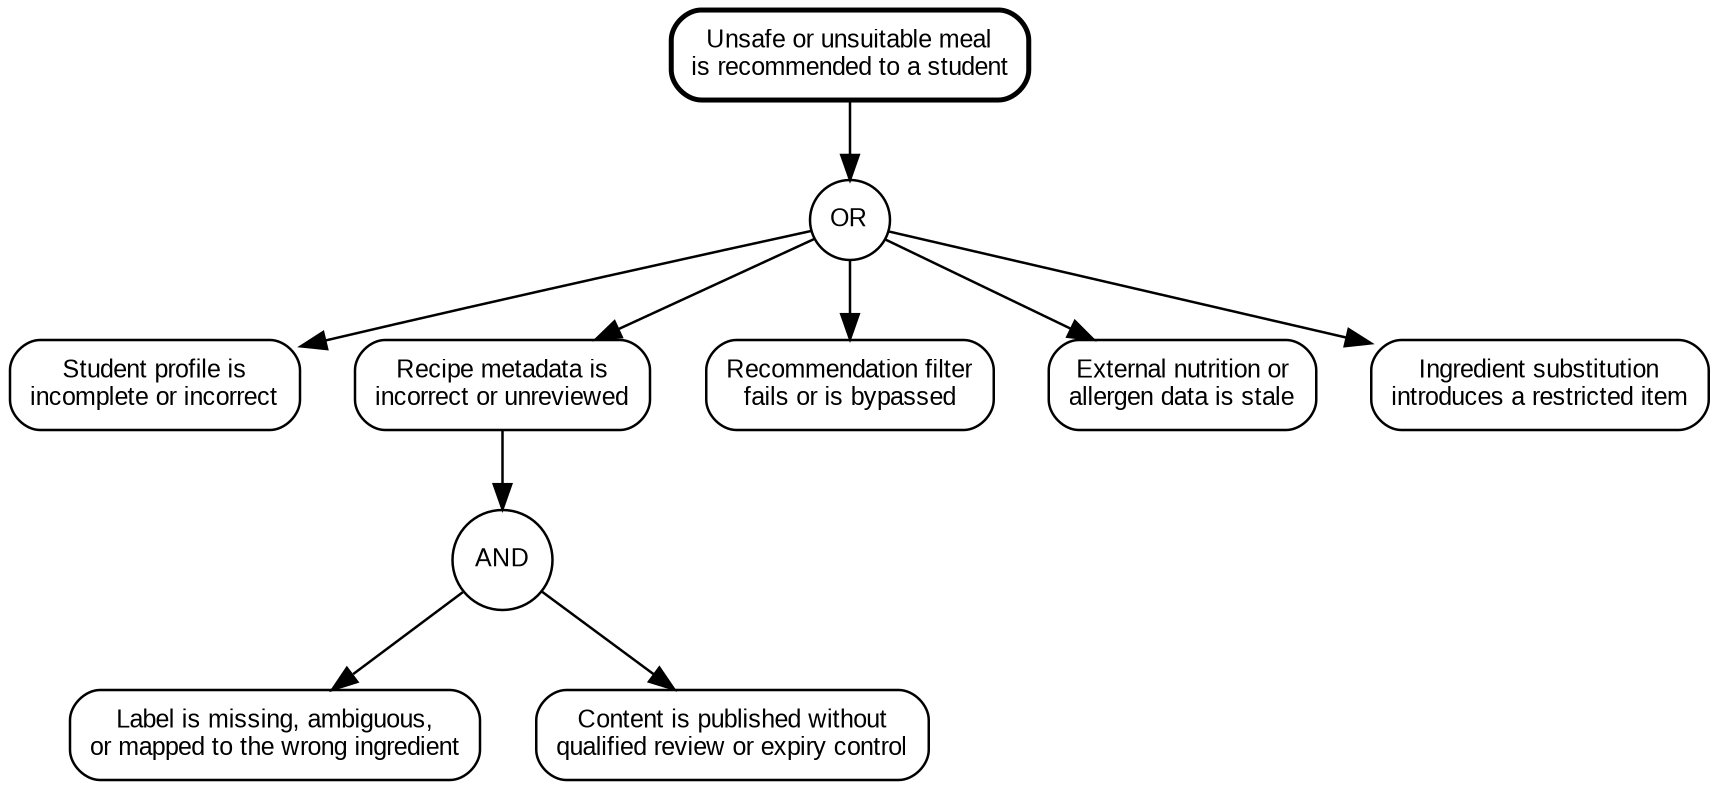
\includegraphics[width=0.96\textwidth]{risk_tree.png}
\caption{Risk tree for unsafe or unsuitable meal recommendation.}
\label{fig:risk-tree}
\end{figure}

\subsection{Consolidated Risk Register and Quantitative Assessment}

\begin{landscape}
\begin{center}
\scriptsize
\setlength{\tabcolsep}{2.5pt}
\renewcommand{\arraystretch}{1.18}
\rowcolors{2}{rowblue}{white}
\begin{longtable}{|p{0.8cm}|p{3.2cm}|p{5.1cm}|p{1.4cm}|p{8.0cm}|p{1.6cm}|p{1.3cm}|p{1.8cm}|}
\hline
\rowcolor{headerblue} \textbf{\color{white}{ID}} & \textbf{\color{white}{Type}} & \textbf{\color{white}{Risk event}} & \textbf{\color{white}{Likelihood}} & \textbf{\color{white}{Likelihood rationale}} & \textbf{\color{white}{Severity (1, 3, 5, 7, 9)}} & \textbf{\color{white}{RE}} & \textbf{\color{white}{Priority}} \\ \hline
\endfirsthead
\hline
\rowcolor{headerblue} \textbf{\color{white}{ID}} & \textbf{\color{white}{Type}} & \textbf{\color{white}{Risk event}} & \textbf{\color{white}{Likelihood}} & \textbf{\color{white}{Likelihood rationale}} & \textbf{\color{white}{Severity (1, 3, 5, 7, 9)}} & \textbf{\color{white}{RE}} & \textbf{\color{white}{Priority}} \\ \hline
\endhead
\hline
\multicolumn{8}{r}{\small\itshape Continued on next page}\\
\endfoot
\hline
\endlastfoot
R1 & Product - data quality & Nutrition or calorie values are incorrect or use inconsistent units. & 0.35 & Several external and manually curated sources may use different serving sizes and update cycles. & 7 & 2.45 & High \\ \hline
R2 & Product - safety & A personalized plan contains an allergen, religiously prohibited item, unsafe substitution, or misleading health-related guidance. & 0.20 & Hard filters and review are intended, but metadata gaps, substitutions, and user-input errors remain credible. & 9 & 1.80 & High* \\ \hline
R3 & Product - affordability & The actual grocery basket exceeds the student's budget. & 0.60 & Prices vary frequently by store, location, tax, package size, promotions, and source freshness. & 5 & 3.00 & High \\ \hline
R4 & Product - security/privacy & Sensitive profile, religious, health, allergy, or budget data is exposed or changed without authorization. & 0.20 & The system is web-based, stores sensitive fields, and defines several privileged roles. & 9 & 1.80 & High* \\ \hline
R5 & Product - availability/reliability & Cloud, database, or external-service failure interrupts planning or causes data loss. & 0.30 & Multiple external services and shared cloud storage create several failure points. & 7 & 2.10 & High \\ \hline
R6 & Product - functional & No feasible plan is generated, or grocery quantities are incomplete because constraints conflict. & 0.35 & Budget, calories, allergies, cuisine, time, skill, and religious rules can make the solution space empty. & 5 & 1.75 & Medium \\ \hline
R7 & Product - usability/accessibility & A student misunderstands profile fields, warnings, nutrition information, or cost uncertainty. & 0.45 & Users have varied technical and cooking skills and may use small mobile screens. & 5 & 2.25 & High \\ \hline
R8 & Process - delivery & The project misses schedule or quality objectives because the scope and integrations are too large. & 0.55 & The Vision Document includes fourteen features plus external services, safety, privacy, moderation, and administration. & 7 & 3.85 & Very High \\ \hline
R9 & Product/process - content governance & Review backlog or weak workflow leaves inaccurate or expired content published. & 0.40 & Qualified review is a dependency, while the number and update frequency of recipes may grow quickly. & 7 & 2.80 & High \\ \hline
\end{longtable}
\rowcolors{2}{}{}
\end{center}
\end{landscape}

\textbf{Severity scale:} 1 is Low; 3 is Medium; 5 is High; 7 is Very High; and 9 is Extreme High. 
\textbf{Priority rule:} $\mathrm{RE}\leq 1.00$ is Low; $1.00<\mathrm{RE}\leq 2.00$ is Medium; $2.00<\mathrm{RE}\leq 3.00$ is High; and $\mathrm{RE}>3.00$ is Very High. A severity of 9 raises the risk to at least High even when exposure is 2.00 or lower. The asterisk marks this severity override.

\subsection{Risk Control Alternatives and RRL}

\begin{landscape}
\begin{center}
\scriptsize
\setlength{\tabcolsep}{2.5pt}
\renewcommand{\arraystretch}{1.18}
\rowcolors{2}{rowblue}{white}
\begin{longtable}{|p{0.7cm}|p{0.6cm}|p{6.0cm}|p{3.2cm}|p{1.1cm}|p{1.1cm}|p{1.3cm}|p{1.3cm}|p{1.1cm}|p{3.0cm}|}
\hline
\rowcolor{headerblue} \textbf{\color{white}{Risk}} & \textbf{\color{white}{Alt.}} & \textbf{\color{white}{Countermeasure}} & \textbf{\color{white}{Tactic}} & \textbf{\color{white}{Residual P}} & \textbf{\color{white}{Residual S}} & \textbf{\color{white}{Residual RE}} & \textbf{\color{white}{Cost points}} & \textbf{\color{white}{RRL}} & \textbf{\color{white}{Decision}} \\ \hline
\endfirsthead
\hline
\rowcolor{headerblue} \textbf{\color{white}{Risk}} & \textbf{\color{white}{Alt.}} & \textbf{\color{white}{Countermeasure}} & \textbf{\color{white}{Tactic}} & \textbf{\color{white}{Residual P}} & \textbf{\color{white}{Residual S}} & \textbf{\color{white}{Residual RE}} & \textbf{\color{white}{Cost points}} & \textbf{\color{white}{RRL}} & \textbf{\color{white}{Decision}} \\ \hline
\endhead
\hline
\multicolumn{10}{r}{\small\itshape Continued on next page}\\
\endfoot
\hline
\endlastfoot
R1 & A & Validate units/ranges, store source metadata, and perform periodic nutrition-advisor sampling. & Reduce risk likelihood & 0.12 & 5 & 0.60 & 4 & 0.463 & Select \\ \hline
R1 & B & Use one authoritative nutrition database only. & Avoid/reduce risk & 0.10 & 5 & 0.50 & 6 & 0.325 & Not selected \\ \hline
R2 & A & Hard allergen/religious filter, unknown-data block, substitution re-check, and automated safety tests. & Avoid risk consequence & 0.06 & 9 & 0.54 & 5 & 0.252 & Select; combine with review \\ \hline
R2 & B & Human pre-publication review without an automated hard block. & Reduce risk likelihood & 0.10 & 9 & 0.90 & 4 & 0.225 & Secondary control \\ \hline
R3 & A & Use timestamped prices, normalized units, a 10\% contingency buffer, and low-confidence warning. & Reduce consequence likelihood & 0.30 & 5 & 1.50 & 2 & 0.750 & Select \\ \hline
R3 & B & Purchase real-time multi-store pricing with broad local coverage. & Reduce risk likelihood & 0.15 & 5 & 0.75 & 7 & 0.321 & Defer \\ \hline
R4 & A & Encrypt data, enforce least-privilege RBAC, privileged-user MFA, and audit logs. & Reduce risk likelihood & 0.07 & 9 & 0.63 & 6 & 0.195 & Select \\ \hline
R4 & B & Add data minimization, field-level encryption, and isolated sensitive-data storage. & Avoid/mitigate consequence & 0.04 & 7 & 0.28 & 8 & 0.190 & Future hardening \\ \hline
R5 & A & Cache read-only data, provide degraded mode, automate backups, and test restoration. & Mitigate consequence & 0.12 & 5 & 0.60 & 4 & 0.375 & Select \\ \hline
R5 & B & Deploy multi-region active redundancy for the complete stack. & Avoid consequence & 0.05 & 5 & 0.25 & 9 & 0.206 & Defer \\ \hline
R6 & A & Validate constraint combinations, explain infeasibility, and let users relax only non-safety preferences. & Reduce risk likelihood & 0.12 & 3 & 0.36 & 3 & 0.463 & Select \\ \hline
R6 & B & Escalate every infeasible case to a support specialist. & Restore/mitigate & 0.20 & 5 & 1.00 & 4 & 0.188 & Backup only \\ \hline
R7 & A & Use an accessible profile wizard, plain-language warnings, usability testing, and input confirmation. & Reduce risk likelihood & 0.20 & 3 & 0.60 & 4 & 0.413 & Select \\ \hline
R7 & B & Provide a help center without redesigning the input workflow. & Mitigate consequence & 0.35 & 5 & 1.75 & 2 & 0.250 & Not selected \\ \hline
R8 & A & Define an MVP and defer lower-priority integrations/features to later releases. & Avoid risk boundary & 0.25 & 5 & 1.25 & 2 & 1.300 & Select \\ \hline
R8 & B & Add developers and a project manager while retaining full scope. & Reduce risk likelihood & 0.30 & 5 & 1.50 & 8 & 0.294 & Not selected \\ \hline
R9 & A & Use draft-review-publish-retire states, review SLA, expiry, audit history, and automatic withdrawal. & Reduce risk likelihood & 0.15 & 5 & 0.75 & 4 & 0.513 & Select \\ \hline
R9 & B & Add moderators without changing the workflow. & Reduce risk likelihood & 0.20 & 5 & 1.00 & 6 & 0.300 & Not selected \\ \hline
\end{longtable}
\rowcolors{2}{}{}
\end{center}
\end{landscape}

The interpretation of the RRL indicates that alternatives are assessed within the same risk framework, as the cost points represent relative effort estimates. A higher RRL results in greater exposure reduction for each unit of effort expended. For R2, safety warrants the implementation of layered controls, despite the automated hard block being the primary choice. For R4, the higher-reduction architecture continues to be a viable option for future hardening, even though it has a slightly lower RRL.

\subsection{Selected Risk-Countermeasure Requirements}

\begin{center}
\small
\setlength{\tabcolsep}{2.5pt}
\renewcommand{\arraystretch}{1.18}
\rowcolors{2}{rowblue}{white}
\begin{longtable}{|p{2.2cm}|p{13.8cm}|}
\hline
\rowcolor{headerblue} \textbf{\color{white}{Requirement ID}} & \textbf{\color{white}{Selected countermeasure requirement}} \\ \hline
\endfirsthead
\hline
\rowcolor{headerblue} \textbf{\color{white}{Requirement ID}} & \textbf{\color{white}{Selected countermeasure requirement}} \\ \hline
\endhead
\hline
\multicolumn{2}{r}{\small\itshape Continued on next page}\\
\endfoot
\hline
\endlastfoot
CM-R1 & The system shall normalize nutrition units and serving sizes, store the source and update date for every nutrition record, reject values outside configured validation ranges, and flag records due for qualified review. \\ \hline
CM-R2 & The system shall prevent a recipe or substitute from entering a personalized plan when any declared allergen is present or when required allergen or religious-compliance metadata is unknown. \\ \hline
CM-R3 & The system shall calculate budget estimates using timestamped normalized prices, apply a configurable contingency buffer of 10\% by default, and display source coverage and uncertainty. \\ \hline
CM-R4 & The system shall encrypt sensitive data in transit and at rest, enforce least-privilege role-based access, require multi-factor authentication for privileged roles, and record access to sensitive fields. \\ \hline
CM-R5 & The system shall provide degraded read-only access to profiles, saved plans, and cached recipes during external-data outages and shall back up application data daily with a quarterly restore test. \\ \hline
CM-R6 & The system shall validate profile constraints before plan generation and, when no feasible plan exists, identify the conflicting constraints without automatically relaxing allergies or religious restrictions. \\ \hline
CM-R7 & At least 90\% of representative student participants shall complete profile setup and weekly-plan generation without assistance during usability testing; all critical warnings shall meet applicable accessibility contrast and keyboard-use criteria. \\ \hline
CM-R8 & Release 1 shall prioritize profile management, safe recipe recommendation, single-student weekly planning, budget estimation, and grocery-list generation; advanced tracking, ratings, email notifications, and full household planning may be deferred. \\ \hline
CM-R9 & Recipe content shall follow draft, review, published, and retired states; publication shall require an authorized reviewer; edits to safety-relevant fields shall trigger re-review; and expired content shall be removed automatically from personalized results. \\ \hline
\end{longtable}
\rowcolors{2}{}{}
\end{center}

\subsection{Residual Risk Summary}

\begin{center}
\small
\setlength{\tabcolsep}{2.5pt}
\renewcommand{\arraystretch}{1.18}
\rowcolors{2}{rowblue}{white}
\begin{longtable}{|p{1.8cm}|p{2.5cm}|p{2.5cm}|p{2.5cm}|p{6.2cm}|}
\hline
\rowcolor{headerblue} \textbf{\color{white}{Risk}} & \textbf{\color{white}{Initial RE}} & \textbf{\color{white}{Residual RE}} & \textbf{\color{white}{Reduction}} & \textbf{\color{white}{Residual treatment}} \\ \hline
\endfirsthead
\hline
\rowcolor{headerblue} \textbf{\color{white}{Risk}} & \textbf{\color{white}{Initial RE}} & \textbf{\color{white}{Residual RE}} & \textbf{\color{white}{Reduction}} & \textbf{\color{white}{Residual treatment}} \\ \hline
\endhead
\hline
\multicolumn{5}{r}{\small\itshape Continued on next page}\\
\endfoot
\hline
\endlastfoot
R1 & 2.45 & 0.60 & 1.85 & Accept with monitoring \\ \hline
R2 & 1.80 & 0.54 & 1.26 & Accept with monitoring \\ \hline
R3 & 3.00 & 1.50 & 1.50 & Additional review required \\ \hline
R4 & 1.80 & 0.63 & 1.17 & Accept with monitoring \\ \hline
R5 & 2.10 & 0.60 & 1.50 & Accept with monitoring \\ \hline
R6 & 1.75 & 0.36 & 1.39 & Accept with monitoring \\ \hline
R7 & 2.25 & 0.60 & 1.65 & Accept with monitoring \\ \hline
R8 & 3.85 & 1.25 & 2.60 & Additional review required \\ \hline
R9 & 2.80 & 0.75 & 2.05 & Accept with monitoring \\ \hline
\end{longtable}
\rowcolors{2}{}{}
\end{center}

The selected controls reduce every residual exposure to 1.25 or lower. R8 remains above 1.00 because schedule risk cannot be eliminated by requirements alone; the MVP scope decision must be enforced through change control. R2 also remains safety-critical despite low residual exposure and therefore requires continuous monitoring, test coverage, content review, and incident response.

\section{Conclusions and Recommended Vision Document Changes}

The Vision Document establishes a coherent student-centered concept, but several high-level statements are too absolute for the stated dependencies and safety context. The most important revisions are to distinguish estimated cost from guaranteed budget compliance, make allergen handling fail-safe, define measurable availability and degraded mode, limit release 1 to single-student nutrition with serving-size scaling, clarify privileged roles and content-review authority, and introduce explicit behavior for infeasible profiles.

The risk assessment identifies scope overrun and price uncertainty as the highest-exposure risks, while allergen safety and privacy require priority treatment because of their severity. The selected countermeasures should be incorporated into the next Vision revision and traced into use cases, supplementary requirements, design decisions, and test cases in Delivery \#3.

\section*{References}

\addcontentsline{toc}{section}{References}

\begin{enumerate}[label={[\arabic*]},leftmargin=2.2em]

\item NourishU Vision Document, version 1.1, Delivery \#1, July 2026.

\item SOEN 6481 Delivery \#2 assignment instructions, Requirements Evaluation and Risk Analysis, Summer 2026.

\item SOEN 6481 Lecture 3, Part 1: Requirements Evaluation and Risk Analysis - inconsistency management, interaction matrices, conflict-resolution operators, risk identification, assessment, control, and RRL.

\item SOEN 6481 Lecture 3, Part 2: Requirements Evaluation and Risk Analysis - weighted matrices and quantitative decision support.

\item G. Kotonya and I. Sommerville, interaction-matrix technique, 1997, as cited in the course materials.

\item A. van Lamsweerde, Requirements Engineering: From System Goals to UML Models to Software Specifications, Wiley, 2009.

\end{enumerate}

\appendix

\section{Task 0 Activity Log}

Complete this table with the actual dates and time personally spent. Do not submit estimated or fabricated hours. The total must match the work recorded in the version history or document-editing platform where possible.

\begin{center}
\small
\setlength{\tabcolsep}{2.5pt}
\renewcommand{\arraystretch}{1.18}
\rowcolors{2}{rowblue}{white}
\begin{longtable}{|p{2.8cm}|p{10.5cm}|p{2.5cm}|}
\hline
\rowcolor{headerblue} \textbf{\color{white}{Date}} & \textbf{\color{white}{Task/activity}} & \textbf{\color{white}{Time spent}} \\ \hline
\endfirsthead
\hline
\rowcolor{headerblue} \textbf{\color{white}{Date}} & \textbf{\color{white}{Task/activity}} & \textbf{\color{white}{Time spent}} \\ \hline
\endhead
\hline
\multicolumn{3}{r}{\small\itshape Continued on next page}\\
\endfoot
\hline
\endlastfoot
18-07-2026 & Task 0 - Set up activity log and report structure & 1 hr. \\ \hline
18-07-2026 & Task 1 - Inspect Vision Document and complete inspection records & 3 hr. \\ \hline
18-07-2026 & Task 2 - Build and interpret interaction matrix & 2 hr. \\ \hline
19-07-2026 & Task 3 - Generate conflict resolutions and revised requirements & 2.5 hr. \\ \hline
19-07-2026 & Task 4 - Define criteria, score alternatives, and select resolutions & 2 hr. \\ \hline
24-07-2026 & Task 5 - Identify, assess, and control risks; calculate RRL & 3 hr. \\ \hline
24-07-2026 & Final review, anonymization, formatting, and submission preparation & 5 hr. \\ \hline
 & Total & 18.5 hrs. \\ \hline
\end{longtable}
\rowcolors{2}{}{}
\end{center}

\section{Traceability from Findings to Decisions}

\begin{landscape}
\begin{center}
\scriptsize
\setlength{\tabcolsep}{2.5pt}
\renewcommand{\arraystretch}{1.18}
\rowcolors{2}{rowblue}{white}
\begin{longtable}{|p{3.4cm}|p{2.4cm}|p{3.2cm}|p{4.3cm}|p{9.0cm}|}
\hline
\rowcolor{headerblue} \textbf{\color{white}{Inspection findings}} & \textbf{\color{white}{Conflict}} & \textbf{\color{white}{Selected resolution}} & \textbf{\color{white}{Revised requirement}} & \textbf{\color{white}{Risk/countermeasure trace}} \\ \hline
\endfirsthead
\hline
\rowcolor{headerblue} \textbf{\color{white}{Inspection findings}} & \textbf{\color{white}{Conflict}} & \textbf{\color{white}{Selected resolution}} & \textbf{\color{white}{Revised requirement}} & \textbf{\color{white}{Risk/countermeasure trace}} \\ \hline
\endhead
\hline
\multicolumn{5}{r}{\small\itshape Continued on next page}\\
\endfoot
\hline
\endlastfoot
F04 & C1 & C1-C & BR-3 & R3 / CM-R3 \\ \hline
F07-F09 & C2 & C2-B & SA-2 & R1, R2, R9 / CM-R1, CM-R2, CM-R9 \\ \hline
F05 & C3 & C3-A & AV-1 & R5 / CM-R5 \\ \hline
F01, F06 & C4 & C4-A & EX-1 & R1, R3, R5 / CM-R1, CM-R3, CM-R5 \\ \hline
F03 & C5 & C5-B & HH-2 & R6, R8 / CM-R6, CM-R8 \\ \hline
F02, F11, F14-F16 & Supporting revisions & N/A & Role, security, administration, and workflow clarifications & R4, R5, R9 / CM-R4, CM-R5, CM-R9 \\ \hline
\end{longtable}
\rowcolors{2}{}{}
\end{center}
\end{landscape}

\end{document}